\subsection{CI/CD chains}

We use CircleCI as a continous integration and continous delivery platform, and have configured a workflow \cite{workflow:circleci} with jobs to build, test, and deploy our service, generate a changelog, as well as building our \LaTeX\ project. At the end of this section, there is a diagram (\autoref{fig:ci-cd-diagram}) showing our full CI/CD flow.

\subsubsection{Building, testing, and static analysis}

This part of the workflow quite simply installs the dependencies, and then builds and tests the project. Additionally it runs the following three static code analysis jobs:
\begin{itemize}
    \item A Go linters runner: \texttt{golangci-lint}, which runs dozens of linters in parallel.
    \item A cyclomatic complexity calculator: \texttt{gocyclo}, to ensure that the code has low complexity. Otherwise, the job will exit with code 1 until we've refactored the functions in question.
    \item A developer security platform, \texttt{Snyk}, to find and fix security vulnerabilities in code, dependencies, and containers.
\end{itemize}


\subsubsection{Deploying our service}

CircleCI will also:
\begin{itemize}
    \item Publish a GitHub release
    \item Push our changes to the four images in Docker Hub (the server, front-end, Prometheus, and Grafana)
    \item Deploy to their respective images in the managed Kubernetes service in the remote Azure server
    \item Apply infrastructure via Terraform
\end{itemize}


\subsubsection{Generating a changelog, and building the \LaTeX\ project}

We use CircleCI Github Changelog Generator \cite{tool:changelog-generator} to generate a changelog based on our tags, issues, labels and pull requests on GitHub.

In order to include a build of the \LaTeX\ project in the CircleCI workflow, we've written a script to let CircleCI run a custom Docker image, build a PDF, and then commit it to the branch.

\begin{figure}[H]
    \makebox[\textwidth][c]{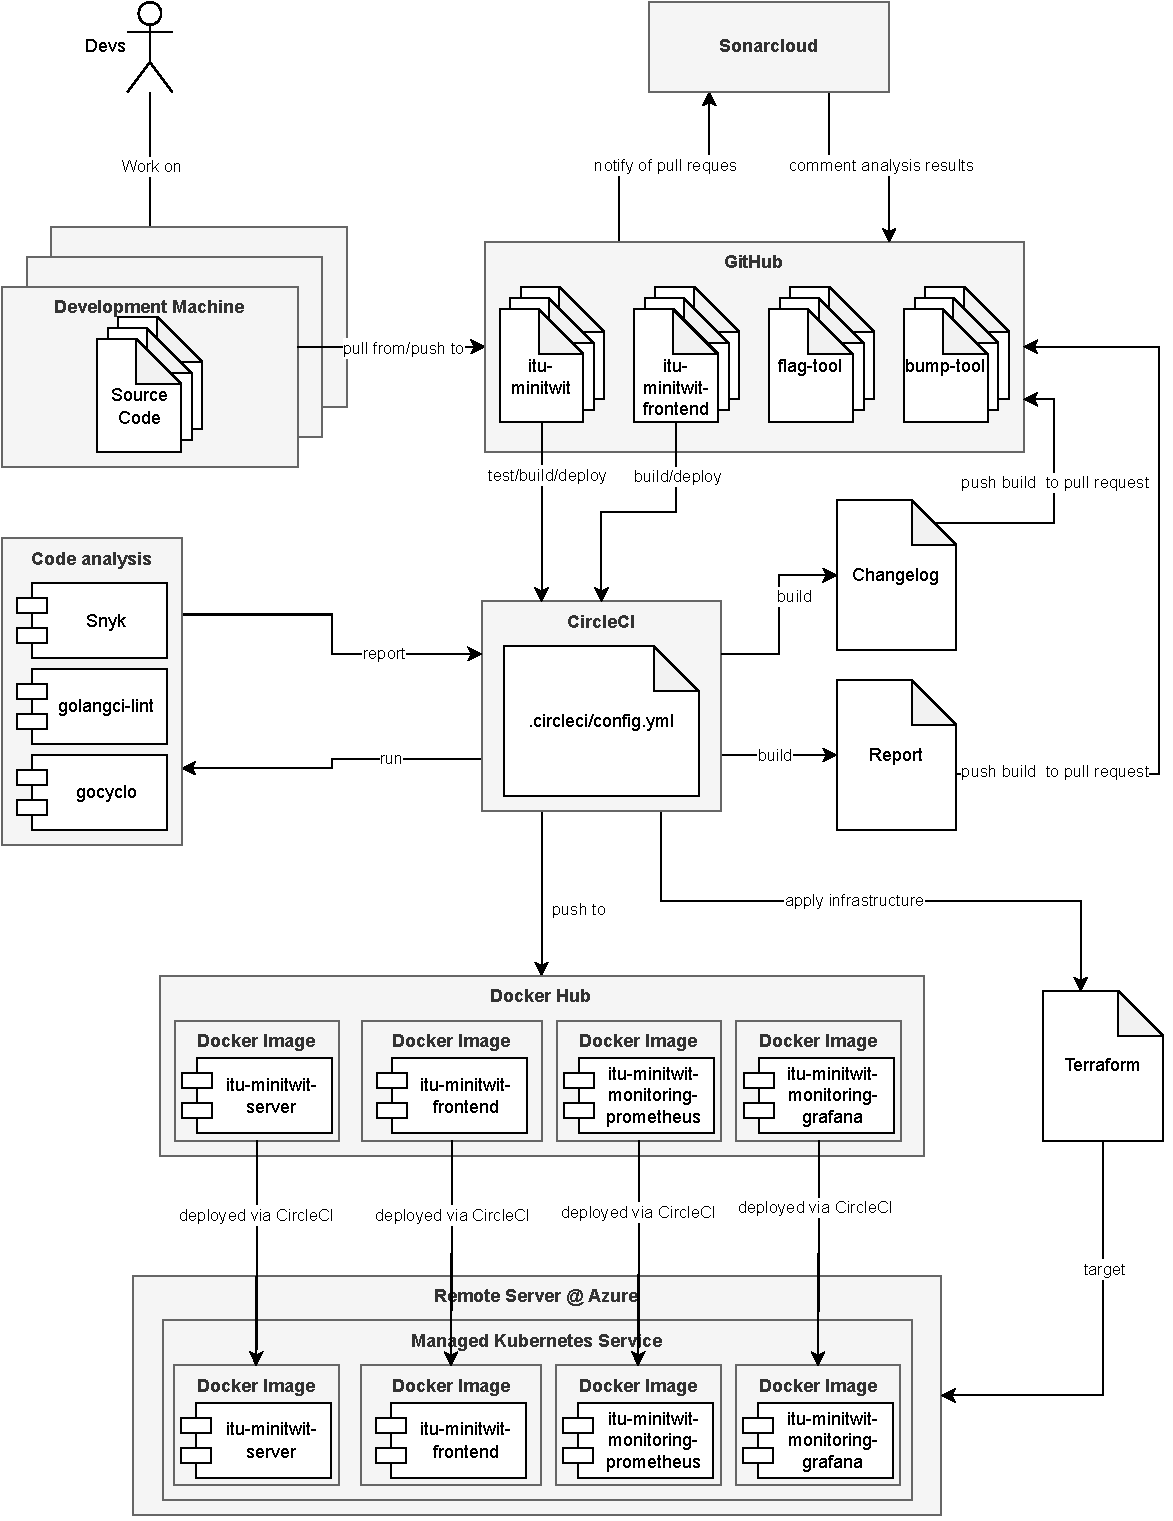
\includegraphics[width=0.85\paperwidth]{workflow}}%
    \caption{A diagram showing our CI/CD flow.}
    \label{fig:ci-cd-diagram}
\end{figure}
